\documentclass{standalone}
\usepackage{graphicx}
\usepackage{tikz}
\usetikzlibrary{shapes.geometric}


\begin{document}
\begin{tikzpicture}
	\node[anchor=south west,inner sep=0] (image) at (0,0,0) {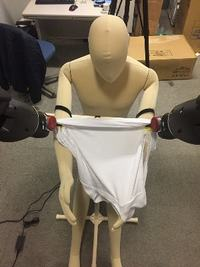
\includegraphics[width=\linewidth]{2}};
	\begin{scope}[x={(image.south east)},y={(image.north west)}]
		\iffalse
		% Next four lines helps to locate the point needed by forming a grid
		\draw[help lines,xstep=.1,ystep=.1] (0,0) grid (1,1);
		\draw[help lines,xstep=.05,ystep=.05] (0,0) grid (1,1);
		\foreach \x in {0,1,...,9} {\node[anchor=north] at (\x/10,0) {0.\x}; }
		\foreach \y in {0,1,...,9} {\node[anchor=east] at (0,\y/10) {0.\y};}
		\fi
		\begin{scope}[x={(image.south east)},y={(image.north west)}]
			\draw (0.48,0.2) node[ellipse, ultra thick, draw=red,minimum height=80pt,minimum width=150pt] {};
		\end{scope}
	\end{scope}
\end{tikzpicture}
\end{document}
